\documentclass[crop, tikz]{standalone}
\usepackage{tikz}

\usetikzlibrary{calc}
\usepackage{colortbl}

 
 % Definition of circles
\def\square{(-2,-2) rectangle (4,2)}
\def\firstcircle{(0,0) circle (1.5cm)}
\def\secondcircle{(0:2cm) circle (1.5cm)}

\colorlet{circle edge}{black}
\colorlet{circle area}{gray!30!blue!20}

\colorlet{circle edge2}{black!80}
\colorlet{circle area2}{blue}


\tikzset{filled/.style={fill=circle area, draw=circle edge, thick},
	filled2/.style={fill=circle area2, draw=circle edge2, thick},
    outline/.style={draw=circle edge, thick}}

\setlength{\parskip}{5mm}
 
 \begin{document}

 
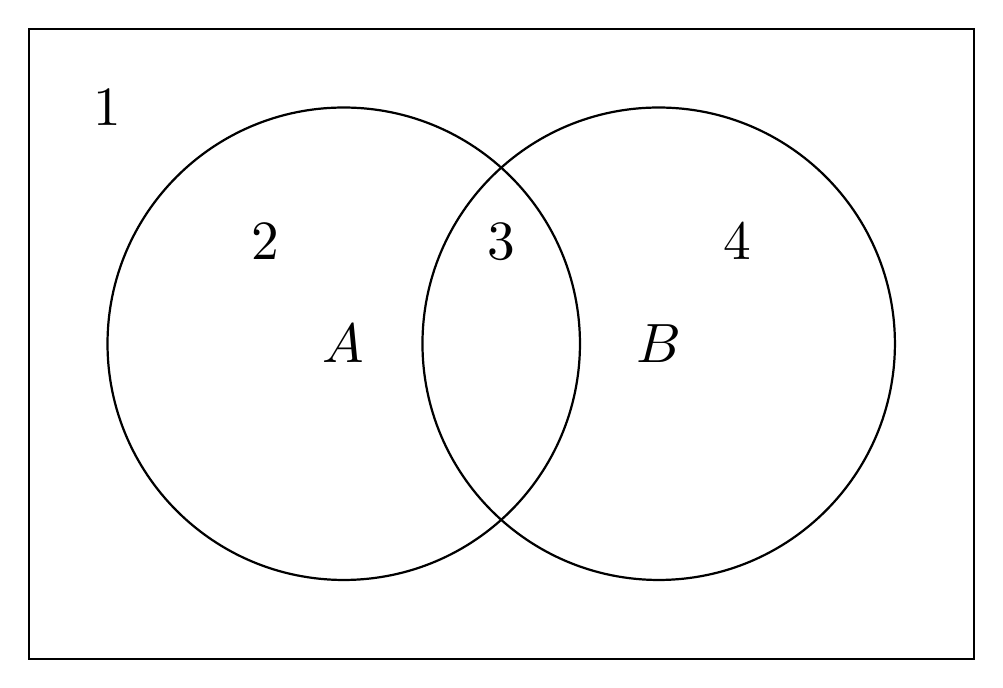
\begin{tikzpicture}[scale=2, transform shape] 
 
 \node at (-1.5,1.5) {$1$}; 
 \node at (-0.5,0.65) {$2$}; 
 \node at (1, 0.65) {$3$}; 
  \node at (2.5, 0.65) {$4$}; 

\draw[outline] \firstcircle node  {$A$};
\draw[outline] \secondcircle node  {$B$};
 \draw[outline] \square; 
 % \node[anchor=south] at (current bounding box.north) {$P\wedge \neg P$};

\end{tikzpicture}
 
\end{document}
